\documentclass[a4paper, 11pt]{article}
\usepackage{comment} 
\usepackage{lipsum} %This package just generates Lorem Ipsum filler text. 
\usepackage{fullpage} % changes the margin
\usepackage[a4paper, total={7in, 10in}]{geometry}
\usepackage[fleqn]{amsmath}
\usepackage{amssymb,amsthm}  % assumes amsmath package installed
\newtheorem{theorem}{Theorem}
\newtheorem{corollary}{Corollary}
\usepackage{graphicx}
\usepackage{tikz}
\usetikzlibrary{arrows}
\usepackage{verbatim}
\usepackage[numbered]{mcode}
\usepackage{float}
\usepackage{tikz}
    \usetikzlibrary{shapes,arrows}
    \usetikzlibrary{arrows,calc,positioning}

    \tikzset{
        block/.style = {draw, rectangle,
            minimum height=1cm,
            minimum width=1.5cm},
        input/.style = {coordinate,node distance=1cm},
        output/.style = {coordinate,node distance=4cm},
        arrow/.style={draw, -latex,node distance=2cm},
        pinstyle/.style = {pin edge={latex-, black,node distance=2cm}},
        sum/.style = {draw, circle, node distance=1cm},
    }
\usepackage{xcolor}
\usepackage{mdframed}
\usepackage[shortlabels]{enumitem}
\usepackage{indentfirst}
\usepackage{hyperref}
\usepackage[capitalize, nameinlink]{cleveref}
\renewcommand{\thesubsection}{\thesection.\alph{subsection}}

\newenvironment{problem}[2][Problem]
    { \begin{mdframed}[backgroundcolor=gray!20] \textbf{#1 #2} \\}
    {  \end{mdframed}}

\newenvironment{reduction}
    { \begin{mdframed}[backgroundcolor=blue!20] \\}
    {  \end{mdframed}}
% Define solution environment

\newcommand{\hr}{\noindent\rule{7in}{2.8pt}}
\newenvironment{solution}
    {\textit{Solution:}}
    {\clearpage}
\newcommand{\prob}[1]{\begin{mdframed}[backgroundcolor=gray!20] \textbf{Problem #1}\end{mdframed}}
\renewcommand{\qed}{\quad\qedsymbol}
\newcommand{\bit}{\left\{0, 1\right\}}
\newcommand{\enc}{\mathsf{Enc}}
\newcommand{\dec}{\mathsf{Dec}}
\newcommand{\poly}{\mathsf{poly}}
\newcommand{\N}{\mathbb{N}}
\newcommand{\R}{\mathbb{R}}
\newcommand{\Z}{\mathbb{Z}}

\newcommand{\calA}{\mathcal{A}}
\newcommand{\calB}{\mathcal{B}}
\newcommand{\calC}{\mathcal{C}}
\newcommand{\calE}{\mathcal{E}}
\newcommand{\calF}{\mathcal{F}}
\newcommand{\calG}{\mathcal{G}}
\newcommand{\calH}{\mathcal{H}}
\newcommand{\calK}{\mathcal{K}}
\newcommand{\calM}{\mathcal{M}}
\newcommand{\calS}{\mathcal{S}}
\newcommand{\calX}{\mathcal{X}}
\newcommand{\calY}{\mathcal{Y}}

\newcommand{\inparen}[1]{\left{ #1 \right}}
\newcommand{\probtwo}[2]{\mathsf{Pr}_{#1}\left[ #2 \right]}
\newcommand{\set}[1]{\left\{ #1 \right\}}
\newcommand{\ct}{\mathsf{ct}}
\newcommand{\twotimessadv}[1]{\mathsf{2SSAdv}\left[ #1 \right]}



\newlength{\protowidth}
\newcommand{\pprotocol}[5]{
{\begin{figure*}[#3]
\begin{center}
\setlength{\protowidth}{\textwidth}
\addtolength{\protowidth}{-3\intextsep}

\fbox{
        \small
        \hbox{\quad
        \begin{minipage}{\protowidth}
    \begin{center}
    {\bf #1}
    \end{center}
        #5
        \end{minipage}
        \quad}

        }
        
\end{center}
\vspace{-4ex}
\caption{{#4} #2}
\end{figure*}
} }

% the first arg is name of security game
% the second arg is caption
% the third arg is the game description
% the label needs to be included 
\newcommand{\securitygame}[4]{
   \pprotocol{#1}{#2}{tbh!}{#3}{#4}
}

\newcommand{\constr}[4]{
   \pprotocol{#1}{#2}{tbh!}{#3}{#4}
}

\begin{document}

\noindent
\large\textbf{Anish Banerjee, Shankh Gupta} \hfill \textbf{Problem Set - 1}   \\
\normalsize COL759: Cryptography \hfill August 2023\\
\hr


\prob{1: Perfect 2 time security}
\begin{solution}

\end{solution}


\prob{2 : Secure/Insecure PRGs and PRFs}
\begin{solution}
    \begin{enumerate}[(a)]
        \item PRGs
        \begin{enumerate}[i.]
            \item $\calG' = \set{G'_n : \bit^{2n} \to \bit^{3n}}_{n \in \N}$, where $$ G'_n(s_1 ~||~ s_2) = G_n(s_1) \wedge G_n(s_2).$$ 
            The given PRG is \textbf{insecure}. As discussed in class and Quiz 2, a secure PRG $G$ can disclose some of the bits of the seed $s$. For convenience we take $n$ to be even but a similar logic can be used for the odd case too. Suppose $G:\bit^n\rightarrow\bit^{3n}$ is such that it reveals the first $n/2$ of its bits: $$G(s_1 ~||~ s_2)=s_1 ~||~ G''(s_2)$$ where $G'':\bit^{n/2}\rightarrow\bit^{5n/2}$ is a secure PRG. It can be proved that $G$ is secure if $G''$ is secure. Now, 
            $$G'(s_1 ~||~ s_2)=G_n(s_{11} ~||~ s_{12}) \wedge G_n(s_{21} ~||~ s_{22})=s_{11}\wedge s_{21} ~||~ G''(s_{12})\wedge G''(s_{22})$$
            which reveals the bits of  $s_{11}\wedge s_{21}$. The advantage of the adversary which exploits this will be close to 1.

            %%%%%%%%%%%%%%%%%%%%%%%%% TODO

            \item $\calG' = \set{G'_n : \bit^{2n} \to \bit^{3n}}_{n \in \N}$, where $$ G'_n(s_1 ~||~ s_2) = G_n(s_1) \oplus G_n(s_2).$$  
        \end{enumerate}
        \item PRFs
        \begin{enumerate}[i.]
            \item $\calF' = \set{F'_n:\bit^{n} \times \bit^{2n} \to \bit^{n}}_{n\in \N}$ where $$F'_n(k, (x_1, x_2)) = F_n(k, x_1) \oplus F_n(k, x_2).$$  
            
            The given family $\calF'$ is \textbf{insecure}. Consider a PPT attacker $\calA$ who sends $\poly(\lambda)$ distinct $(x_i,x_i)$ queries to the  challenger. If the challenger chooses $b=0$ then it will end up sending $$F_n(k, x_i) \oplus F_n(k, x_i)=0^n$$ for each of the queries. The attacker outputs 0 if all the responses are 0 and 1 otherwise. Advantage of the attacker is close to 1, precisely $1-2^{-n\poly(\lambda)}$.

            \item $\calF' = \set{F'_n:\bit^{n} \times \bit^{n} \to \bit^{n}}_{n\in \N}$ where $$F'_n(k, x) = F_n(k, x) \oplus x.$$
            
            The given family is secure. Given an adversary $\calA$ which breaks PRF security of $\calF'$, we can construct an adversary $\calB$ which breaks the security of $\calF$ (\cref{red:p2bii})
            \securitygame{Problem 2(b)(ii)}{Reduction for Problem 2(b)(ii)}{\label{red:p2bii}}
    {
        \begin{itemize}
           \item Challenger picks a uniformly random bit $b \gets \bit$ and a seed $s\gets \bit^n$.
           \item The adversary $\calA$ makes polynomially many queries to $\calB$, who passes them to the challenger. Challenger replies as in the PRF Game.
           \item Upon receiving the response $y_i$ of each query, $\calB$ sends $ y_i\oplus x_i$ to $\calA$
           \item After polynomially many queries, $\calB$ forwards the response send by $\calA$ $(b')$ and wins if $b=b'$.
        \end{itemize}
        }
        
        \end{enumerate}
    \end{enumerate}
    
\end{solution} 

\prob{3 : PRG Security does not imply Related-Key-PRG Security}
\begin{solution}

\end{solution} 


\prob{4 : Constructing PRFs from PRGs}
\begin{solution}
    We will use a tree construction similar to the one given in the book for proving (\cref{fig:TC})
    \begin{figure}[!ht]
        \centering
        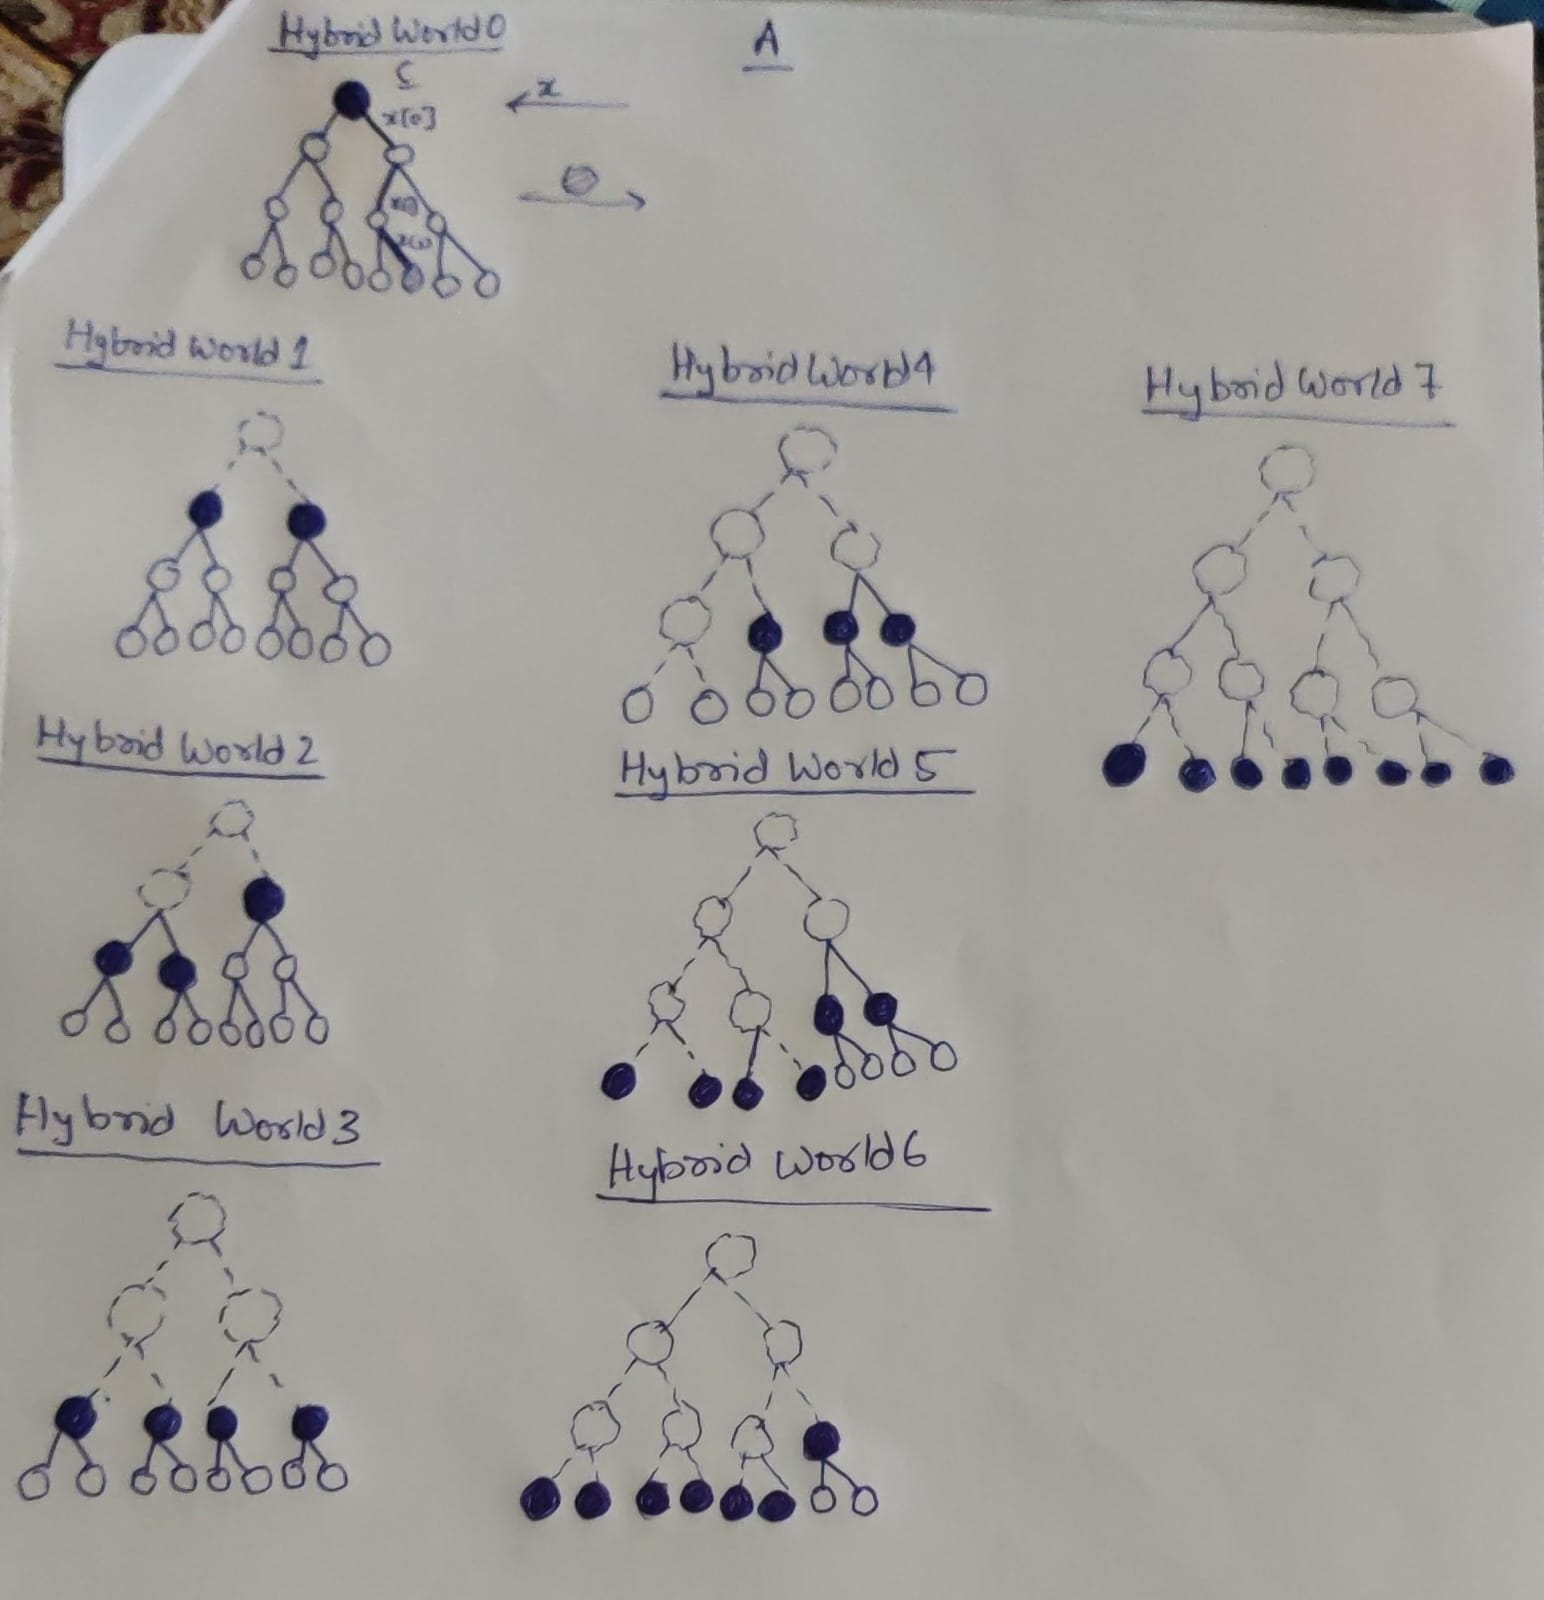
\includegraphics[scale=0.5]{images/Tree Construction.png}
        \caption{Tree construction in the book}
        \label{fig:TC}
    \end{figure}
\begin{enumerate}[(a)]
    \item  Construct $\log n$ hybrid worlds in the following way: in Hybrid world $j$, the challenger samples $2^j$ random bitstrings $s_1, s_2,s_3\dots s_j \gets \bit^n$. Then it applies 
\end{enumerate}
\end{solution} 


\end{document}
 